\documentclass[../../../analisi-dei-requisiti.tex]{subfiles}

\begin{document}

\subsubsection{UUC8: Collegamento organizzazione}%
\label{subs:UUC8}

\begin{figure}[H]
  \centering
  \scalegraphics{collegamento-organizzazione.png}
  \caption{UUC8: Collegamento organizzazione}%
  \label{fig:UUC8}
\end{figure}



\begin{description}
  \item[Caso d’uso:] UUC8;
  \item[Titolo:] Collegamento organizzazione;
  \item[Attori primari:] utente autenticato;
  \item[Precondizione:] l'utente si trova sulla lista delle organizzazioni;
  \item[Postcondizione:] l'utente si collega a un'organizzazione;
  \item[Scenario principale:]
        \begin{enumerate}
          \item l'utente sceglie l'organizzazione alla quale collegarsi.
        \end{enumerate}
\end{description}

\subsubsection{UUC9: Collegamento organizzazione pubblica}%
\label{subs:UUC9}

\begin{description}
  \item[Caso d’uso:] UUC9;
  \item[Titolo:] Collegamento organizzazione pubblica;
  \item[Attori primari:] utente autenticato;
  \item[Precondizione:] l'utente si trova sulla lista delle organizzazioni;
  \item[Postcondizione:] l'utente si collega a un'organizzazione pubblica;
  \item[Scenario principale:]
        \begin{enumerate}
          \item l'utente sceglie l'organizzazione pubblica alla quale collegarsi.
        \end{enumerate}
\end{description}

\subsubsection{UUC10: Collegamento organizzazione privata}%
\label{subs:UUC10}

\begin{figure}[H]
  \centering
  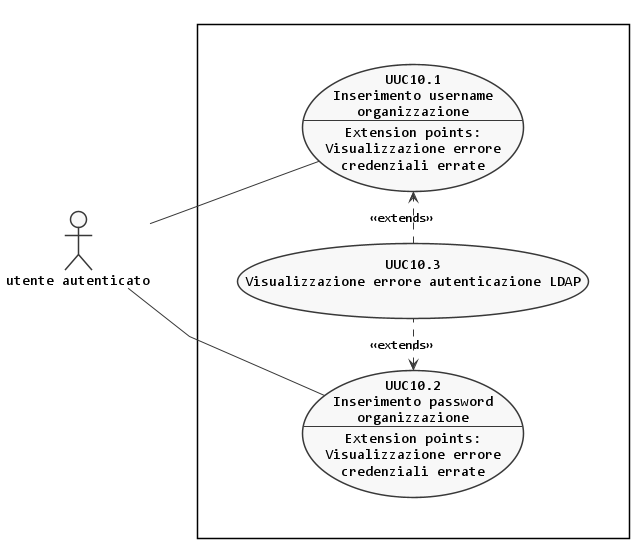
\includegraphics[width=100mm]{autenticazione-ldap-organizzazione.png}
  \caption{UUC10: Collegamento organizzazione }%
  \label{fig:UUC10}
\end{figure}

\begin{description}
  \item[Caso d’uso:] UUC10;
  \item[Titolo:] Collegamento organizzazione privata;
  \item[Attori primari:] utente autenticato;
  \item[Precondizione:] l'utente si trova sulla lista delle organizzazioni;
  \item[Postcondizione:] l'utente si collega a un'organizzazione privata;
  \item[Scenario principale:]
        \begin{enumerate}
          \item l'utente sceglie l'organizzazione privata alla quale collegarsi.
        \end{enumerate}
\end{description}

\subsubsection{UUC10.1: Inserimento username organizzazione}%
\label{subs:UUC10.1}
\begin{description}
  \item[Caso d’uso:] UUC10.1;
  \item[Titolo:] Inserimento username organizzazione;
  \item[Attori primari:] utente autenticato;
  \item[Precondizione:] l'utente ha scelto un'organizzazione privata e non ha ancora inserito lo username dell'organizzazione;
  \item[Postcondizione:] l'utente ha inserito lo username dell'organizzazione privata;
  \item[Scenario principale:]
        \begin{enumerate}
          \item l'utente inserisce lo username relativo all'organizzazione privata alla quale vuole collegarsi;
        \end{enumerate}
  \item[Estensioni:]
        \begin{enumerate}
          \item se lo username inserito dall'utente non corrisponde a quello dell'organizzazione privata, allora visualizzerà un errore~\ref{subs:UUC10.3}.
        \end{enumerate}
\end{description}

\subsubsection{UUC10.2: Inserimento password organizzazione}%
\label{subs:UUC10.2}
\begin{description}
  \item[Caso d’uso:] UUC10.2;
  \item[Titolo:] Inserimento password organizzazione;
  \item[Attori primari:] utente autenticato;
  \item[Precondizione:] l'utente ha scelto un'organizzazione privata e non ha ancora inserito la password dell'organizzazione;
  \item[Postcondizione:] l'utente ha inserito la password dell'organizzazione privata;
  \item[Scenario principale:]
        \begin{enumerate}
          \item l'utente inserisce la password relativa all'organizzazione privata alla quale vuole collegarsi;
        \end{enumerate}
  \item[Estensioni:]
        \begin{enumerate}
          \item se la password inserita dall'utente non corrisponde a quella dell'organizzazione privata, allora visualizzerà un errore~\ref{subs:UUC10.3}.
        \end{enumerate}
\end{description}

\subsubsection{UUC10.3: Visualizzazione errore autenticazione LDAP}%
\label{subs:UUC10.3}
\begin{description}
  \item[Caso d’uso:] UUC10.3;
  \item[Titolo:] Visualizzazione errore autenticazione LDAP\@;
  \item[Attori primari:] utente autenticato;
  \item[Precondizione:] i dati forniti dall'utente non corrispondono a credenziali valide;
  \item[Postcondizione:] l'applicazione mobile comunica all'utente il fallimento dell'autenticazione;
  \item[Scenario principale:]
        \begin{enumerate}
          \item l'utente cerca di effettuare l'autenticazione LDAP all'organizzazione privata con credenziali errate.
        \end{enumerate}
\end{description}


\end{document}
